% CSC 586F Interim Report 2. Build with tectonic from report/ (see README).
% The IR1 numbers quoted in Sections 3 and 4 come from report/data/ir1_results.json (Colab T4, Oct 13).
% The IR2 measurements live in generated/ir2_experiments.tex, written from the IR2 results file.
\documentclass[sigconf,nonacm]{acmart}
\usepackage{booktabs}
\usepackage{graphicx}
\usepackage{xcolor}

\newcommand{\TBD}[1]{\textcolor{red}{\textbf{TBD\if\relax\detokenize{#1}\relax\else: #1\fi}}}
\newcommand{\code}[1]{\texttt{#1}}
\newcommand{\file}[1]{{\urlstyle{tt}\nolinkurl{#1}}}   % file paths, may break at / and .

\settopmatter{printfolios=true}
\setlength{\textfloatsep}{8pt plus 2pt minus 2pt}
\setlength{\dbltextfloatsep}{8pt plus 2pt minus 2pt}
\emergencystretch=1.5em
\raggedbottom

\begin{document}

\title{Pseudo-Bulk RNA-seq Generation on the GPU}
\subtitle{CSC 586F Interim Report 2, Group 19}
\author{Jason Thomo}
\affiliation{%
  \institution{University of Victoria}
  \city{Victoria}
  \state{BC}
  \country{Canada}}
\email{jthomo@uvic.ca}

\begin{abstract}
Interim Report 1 built a gather kernel that computes $P$ pseudo-bulk RNA-seq profiles, the sparse
product $PB = S X^{\top}$, in a few milliseconds on a T4. This report profiles that code and finds
two limits. End to end, 93\% of the time is a host-side data layout step, not the kernel. Inside the
kernel, the SM and the L1 cache are the busy units, not DRAM, because every nonzero costs a dependent
mask lookup, 32 masked adds and a large share of warp shuffles. I propose three ideas backed by that
analysis, estimate the gain of each, and implement and measure all three. Building the layout on
the GPU is 12 to 15 times faster and cuts the medium pipeline from 670 ms to 130 ms. A fused mask stream
with a transposed warp reduction makes the kernel 1.4 to 1.8 times faster on small and medium inputs,
after a first version that spilled to local memory. A complement-based kernel cuts the adds 3.3 times
but runs 2 times slower, and the profile shows why: shared-memory accumulators cost occupancy. Code: \url{https://github.com/jasont7/pbulk-cuda}.
\end{abstract}

\maketitle

\section{Introduction}

Single-cell RNA sequencing gives a sparse gene-by-cell matrix. A \emph{pseudo-bulk} sums the
expression of a set of cells to imitate a bulk tissue sample. Pseudo-bulks are the standard test data
for cell-type deconvolution~\cite{avilacobos2020} and the standard way to run differential expression
across donors~\cite{squair2021,crowell2020}. My research pipeline builds 900 of them from 14,378 genes
by 241,924 cells of 30 donors with an R script that takes about 17 minutes on the Narval cluster.

Interim Report 1 (IR1) gave two CUDA kernels. \code{pb\_scatter} adds every selected nonzero into the
output with atomics. \code{pb\_gather} reorders the data so that one warp owns one (gene, donor)
segment and adds each nonzero into $K$ register accumulators chosen by a bit mask. On synthetic data
with the structure of the real data, gather was 15 to 40 times faster than scatter as a kernel.

This report is the second milestone. Section~\ref{sec:analysis} profiles the IR1 code with Nsight
Compute and a PRAM count. Section~\ref{sec:ideas} turns the analysis into three ideas, each with an
estimate of its gain and its relation to the literature. Section~\ref{sec:impl} describes how they
were built, and Section~\ref{sec:exp} measures them. All data is still synthetic.

\section{Background}

There are $G$ genes, $C$ cells and $D$ donors, and each cell belongs to one donor. $X$ is a sparse
$G \times C$ matrix of CPM values with $N$ nonzeros. Each donor gets $K$ pseudo-bulks, $P = DK$ in
total. The 0/1 selection matrix $S$ ($P \times C$) has $S[p,c] = 1$ when cell $c$ is in pseudo-bulk
$p$, and row $p = dK + k$ only selects cells of donor $d$. Pseudo-bulk $k$ of donor $d$ draws a ratio
$r_{dk}$ uniformly from $[0.3, 1]$ and takes $\lfloor r_{dk} n_d \rfloor$ of the donor's $n_d$ cells.
The output is
\begin{equation}
PB[p,g] = \sum_{c\,:\,S[p,c]=1} X[g,c],
\label{eq:pb}
\end{equation}
with each row then scaled to sum to $10^6$. The real shape is $G = 14{,}378$, $C = 241{,}924$,
$D = K = 30$. The sum has $F = \sum_c t_c n_c$ terms, where $t_c$ is the number of pseudo-bulks that
chose cell $c$ and $n_c$ its number of nonzeros. Because $\mathbb{E}[r] = 0.65$, $F \approx 0.65\,KN$.

\paragraph{The IR1 gather layout.} \code{build\_donor\_layout} sorts cells by donor, stores $X$ by gene
(CSR), and records \code{seg\_ptr}$[gD+d]$, the start of the nonzeros of gene $g$ that belong to donor
$d$. $S$ becomes one 32-bit \code{mask} per cell, with bit $k$ set when the cell is in pseudo-bulk $k$
of its donor. \code{pb\_gather} gives one warp to each of the $GD$ segments. Lane $l$ reads nonzeros
$l, l+32, \dots$, loads the value $v$ and the mask $m = \code{mask}[\code{col}[i]]$, and for each of
32 accumulators adds $v$ if bit $k$ of $m$ is set. A \code{\_\_shfl\_down\_sync} tree then sums each
accumulator across the warp and lane 0 writes the $K$ results. This thread mapping is the CSR vector
kernel of Bell and Garland~\cite{bell2008,bell2009}.

\section{Analysis of the IR1 code}
\label{sec:analysis}

\subsection{Where the end-to-end time goes}

IR1 timed the whole path from host arrays to the result back on the host, on the medium instance
(4,000 genes by 50,000 cells, 16.0 million nonzeros). Gather took 548 ms, of which 510.7 ms (93\%) was
the host layout build, about 31 ms the host-to-device copy, 1.6 to 3.1 ms the kernel and 4 ms the copy
back. Scatter took 60 ms in total, and the single-thread C++ reference 296 ms. So the fastest kernel
gave the slowest pipeline. The layout build grows with the input: 99 ms, 514 ms and 2,404 ms on the
small, medium and large instances (3.2, 16.0 and 76.8 million nonzeros), while the kernel takes 1.0,
1.7 and 5.9 ms. The layout is a NumPy and SciPy routine on one CPU core: a CSC column permutation, a
CSC to CSR conversion, and a chunked \code{bincount} over (gene, donor) keys.

\subsection{What limits the kernel}

Table~\ref{tab:ncu} shows Nsight Compute's view of one \code{pb\_gather} launch on the medium
instance. Nsight locks the SM clock at 585 MHz, which is why the duration is longer than the
event-timed 1.7 ms.

\begin{table}[t]
\caption{Nsight Compute on \code{pb\_gather}, medium instance, Colab T4 (IR1 run).}
\label{tab:ncu}
\small
\begin{tabular}{@{}lr@{}}
\toprule
Metric & Value \\
\midrule
Duration (SM clock locked at 585 MHz) & 2.79 ms \\
Compute (SM) throughput & 76.3\% \\
L1/TEX cache throughput & 86.2\% \\
L2 cache throughput & 25.6\% \\
DRAM throughput & 29.2\% \\
Registers per thread & 65 \\
Theoretical / achieved occupancy & 87.5\% / 84.1\% \\
Grid $\times$ block & 30,000 $\times$ 128 \\
\bottomrule
\end{tabular}
\end{table}

\paragraph{Not memory bound.} DRAM runs at 29\% of its peak, so the kernel is not limited by
bandwidth from device memory. The two busy units are the L1/TEX cache (86\%) and the SM pipelines
(76\%). The kernel is bound by on-chip work: instructions and L1 transactions.

\paragraph{The L1 traffic.} Each loop step of a warp issues three loads: \code{val} and \code{col},
which are coalesced (32 consecutive 4-byte words, four 32-byte sectors each), and \code{mask[col[i]]},
which depends on the second load and is scattered. Within a segment the 32 lanes read 32 cells of one
donor in increasing order, but with 8\% density neighbouring nonzeros of a gene are about 12 cells apart,
so the 32 mask reads span roughly 1.5 KB and touch about 48 sectors. The mask array is small
(200 KB on medium) and stays in L2 and L1, which explains why L1 is hot while DRAM is idle. By this
count the mask lookup is about 85\% of the L1 sectors the loop requests.

\paragraph{The arithmetic.} Every nonzero is offered to all 32 accumulators, even though $K = 30$ and
on average only 19.5 bits of a mask are set. The PRAM work of the gather strategy is
$\Theta(KN + PG)$, against $\Theta(F + PG)$ for the sequential algorithm. The kernel does $32N$
masked adds, 512 million on medium.

\paragraph{The reduction.} After the loop, each lane holds 32 partial sums. The IR1 reduction runs five
\code{\_\_shfl\_down\_sync} steps for each of the 32 accumulators, so all 32 lanes execute 160 shuffles
and 160 adds per segment: 5,120 thread-adds where a reduction tree needs 992. On medium the segments
average 133 nonzeros, only about four loop steps per lane, so the reduction is a large share of the
work. In thread-level adds it is 614 million against the loop's 512 million. Most of those adds
produce values that only lane 0 uses.

\paragraph{Registers and occupancy.} The 32 accumulators cost 65 registers per thread. That limits a
128-thread block to 7 resident blocks per SM (28 of 32 warps), hence the 87.5\% theoretical
occupancy, and it rules out 1,024-thread blocks (IR1 had to cap gather blocks at 512).

\paragraph{Summary.} In order of size: (1) the host layout dominates the pipeline, (2) the kernel is
limited by instructions and L1 transactions, and those come from the dependent mask gather, the 32
masked adds per nonzero and the 160-shuffle reduction.

\section{Ideas}
\label{sec:ideas}

\subsection{Idea 1: build the layout on the GPU}

\paragraph{Evidence.} The layout is 93\% of gather's end-to-end time on medium and grows to 2.4 s on
large (Section~\ref{sec:analysis}).

\paragraph{Idea.} Every step of the layout is a data-parallel primitive. (1) Permuting the columns of
the CSC matrix by donor is a segmented gather: the new column pointer is a prefix sum of the permuted
column lengths, and each new nonzero finds its source with a binary search. (2) CSC to CSR is a sparse
transpose, which cuSPARSE provides~\cite{cusparse}. (3) Because cells are sorted by donor, the key
$gD + \mathrm{donor}(c)$ is nondecreasing along the CSR arrays, so \code{seg\_ptr} is one vectorised
binary search for the $GD+1$ boundaries, with no sort. (4) The masks are a sum of $2^k$ over the
nonzeros of $S$. The bits of one cell are distinct, so the sum equals the bitwise OR and is exact in
float64. The output is identical to the host layout, so the kernels need no change.

\paragraph{Expected gain.} The steps touch each nonzero a small constant number of times, about 1 GB of
memory traffic on medium, which a T4 moves in a few milliseconds at 320 GB/s~\cite{t4datasheet}. With
library overheads I expect 10 to 30 ms instead of 511 ms on medium. The gather pipeline should then
fall from 548 ms to about 60 to 80 ms, a 7 to 9$\times$ gain, now bounded by the host-to-device copy.

\paragraph{Literature.} GPU sparse transposes and segment construction are standard building blocks
(cuSPARSE~\cite{cusparse}, Merrill and Garland's merge-based work~\cite{merrill2016}). The idea is
engineering, not new. The one problem-specific point is that the donor sort makes the segment keys
sorted for free.

\subsection{Idea 2: complement accumulation (less work)}

\paragraph{Evidence.} The kernel is SM-bound and does $32N$ masked adds, almost half of which add zero.

\paragraph{Idea.} Two changes reduce the work, not just its cost. First, a pseudo-bulk that takes more
than half of its donor's cells is computed by its complement: $PB[p,g] = T_{gd} - \sum_{c \notin p} X[g,c]$,
where $T_{gd}$ is the total of the segment. One extra add per nonzero, for $T_{gd}$, serves every
complemented pseudo-bulk. A per-donor \code{flip} word marks which bits are complemented, and the
kernel reads $m \oplus \code{flip}$. Second, a lane visits only the set bits of that word, with
\code{\_\_ffs}, instead of all 32. The work per nonzero falls from 32 to
$1 + \mathrm{popcount}(m \oplus \code{flip})$.

\paragraph{Expected gain.} With $r \sim U(0.3, 1)$, a bit survives the flip with probability
$q = \min(r, 1-r)$ and $\mathbb{E}[q] = 0.293$. The PRAM work falls from $\Theta(KN)$ to
$\Theta(N(1 + \sum_k q_k))$: 9.8 adds per nonzero instead of 32, 3.3$\times$ less. A warp runs in
lockstep, though, so each loop step costs the \emph{largest} popcount among its 32 lanes. A simulation
of the sampling rule gives a mean popcount of 8.8 but a mean warp maximum of 13.8. Dynamic indices also
force the accumulators out of registers into shared memory, and each add becomes a load, an add and a
store. Counting instructions, I expect the loop to speed up by between 0.8$\times$ (a loss) and
1.3$\times$, far below the 3.3$\times$ cut in work. The idea is worth testing because it is the only
one of the three that changes the asymptotic work, and because the gap between the work cut and the
time cut is itself a measurement of SIMT costs.

\paragraph{Literature.} Exploiting the structure of a 0/1 matrix to share additions is old: the Four
Russians method precomputes sums over groups of rows of a binary matrix~\cite{arlazarov1970}, and
masked sparse products skip work outside a mask~\cite{milakovic2022}. Using a complement so that a
dense selection costs as little as a sparse one I have not found in the pseudo-bulk or SpMV literature.
It relies on knowing the segment total, which the donor layout provides for one add.

\subsection{Idea 3: a fused mask stream and a transposed reduction}

\paragraph{Evidence.} L1/TEX is at 86\%, and the scattered mask lookup makes about 85\% of the loop's L1
sector requests. The reduction does 160 shuffles per segment and is larger than the main loop.

\paragraph{Idea.} (a) \emph{Fused mask stream.} The layout stores \code{mval}$[i] = \code{mask}[\code{col}[i]]$
next to each value. The kernel then reads two coalesced streams, \code{val} and \code{mval}, and no
longer needs \code{col}. The bytes the kernel reads per nonzero fall from 12 (with an L1-resident
4-byte mask lookup) to 8, and the dependent load disappears. (b) \emph{Transposed reduction.} Instead
of reducing each accumulator separately, the warp does a recursive-halving reduce-scatter. At offset
$o = 16, 8, 4, 2, 1$, a lane keeps the half of its live accumulators that matches bit $o$ of its lane
index and swaps the other half with lane $l \oplus o$ through \code{\_\_shfl\_xor\_sync}. After five
steps lane $k$ holds the full sum for pseudo-bulk $k$. That is $16+8+4+2+1 = 31$ shuffles and 31 adds
per lane instead of 160, exactly the 992 thread-adds of a tree, and the $K$ outputs are written by $K$
lanes in one instruction instead of $K$ serial stores by lane 0. An ablation kernel,
\code{pb\_gather\_xr}, has (b) only.

\paragraph{Expected gain.} The reduction's thread-adds fall from 614 million to 119 million on medium,
so total adds fall from 1,126 million to 631 million, 1.8$\times$ fewer. Shuffles also cost more than
adds, and the transposed form adds two selects per step, so I expect 1.3 to 1.6$\times$ from (b). Part
(a) removes most of the L1 traffic. If L1 is the binding limit, the kernel moves to being purely
instruction-bound and I expect a further 1.1 to 1.3$\times$. Together, 1.4 to 2$\times$ on the kernel.

\paragraph{Literature.} Warp-level reductions with shuffles are standard~\cite{cudaguide}. The
transposed form is the recursive-halving reduce-scatter used for MPI collectives~\cite{thakur2005},
applied to the 32 registers of a warp. Precomputing an indirection into the stream is a common
trade of memory for latency. I have not found it applied to pseudo-bulk generation, which so far runs
as CPU sparse algebra in R and Python~\cite{crowell2020,squair2021}.

\section{Implementation}
\label{sec:impl}

All new kernels are in \file{pbulk/kernels.cu} next to the IR1 kernels, which are unchanged. Host code is
in \file{pbulk/gpu.py} and \file{pbulk/layout.py}, and the harness in \file{bench/}. As in IR1, kernels
are compiled with CuPy's \code{RawModule}~\cite{okuta2017}, and each one is checked against a float64
reference before it is timed. The kernels also run on the CPU through the IR1 warp emulator
(\file{tests/emu}), which now models \code{\_\_shfl\_xor\_sync} and \code{\_\_ffs}, so their logic is
tested without a GPU.

\paragraph{Idea 1.} \code{build\_donor\_layout\_xp} takes the array module as a parameter. With CuPy
and \code{cupyx.scipy.sparse} it runs on the device. With NumPy and SciPy it runs on the CPU, which is how
the tests check that its arrays equal the host layout bit for bit. The CSC to CSR step calls cuSPARSE
through \code{cupyx}. The donor codes of the cells are still computed on the host, which is a single
\code{np.unique} over the cell labels.

\paragraph{Idea 2.} \code{pb\_gather\_cs} keeps one warp per segment and 128-thread blocks. A lane's
accumulators live in shared memory because their index is only known at run time. Each warp owns a
$32 \times 33$ array of floats, row $k$ and column $l$ holding lane $l$'s sum for bit $k$, so a block
uses 16.5 KB. The final step has lane $k$ sum row $k$. With a row stride of 32 all lanes would hit the
same bank at once. Padding the stride to 33 puts lane $k$ in bank $(k + j) \bmod 32$ at step $j$, so the
read is conflict-free. During accumulation the lanes write to arbitrary rows, so conflicts there depend
on the data, which the experiments measure. The segment total $T_{gd}$ is a register reduced with five
shuffles, and lane $k$ writes $T_{gd} - s_k$ for a flipped bit and $s_k$ otherwise. The flip words come
from the selection counts and add $4D$ bytes.

\paragraph{Idea 3.} \code{pb\_gather\_fm} reads \code{mval} instead of \code{col} and \code{mask}, and
uses the transposed reduction. The loops over accumulators are fully unrolled with compile-time
indices, so all 32 accumulators stay in registers through the reduction. I chose not to stage the
masks in shared memory, which was the other way to cut L1 traffic. A block would have to hold a whole
donor's masks, up to 32 KB at the real shape, which caps occupancy, and the segments of one block
would have to come from one donor. The fused stream needs no shared memory and no
\code{\_\_syncthreads()}, at the cost of 4 bytes per nonzero of device memory.

\paragraph{Launch shape.} All gather variants keep 128-thread blocks. At 65 registers per thread a
block needs 8,320 registers, so 7 blocks fit an SM. Larger blocks give the scheduler nothing extra
because warps never cooperate across a block, except in \code{pb\_gather\_cs}, where shared memory
(16.5 KB per block) allows at most 3 blocks per SM even with the largest 64 KB carve-out.

\paragraph{Library baseline.} For comparison with a vendor library, the harness also computes
$S X^{\top}$ as a cuSPARSE sparse-sparse product through \code{cupyx}, with $S$ as a float32 CSR
matrix~\cite{cusparse}.

\paragraph{Effort and limitations.}
I checked every kernel against the reference and the emulator, and every number in Section~\ref{sec:exp} comes
from two Colab runs: the failed first version of Idea 3 from the first, everything else from the second. Idea 1 was the easiest, because the primitives exist in
CuPy. Idea 2 took the most care: the complement makes the sums the difference of two float32 values, so
it loses a little precision when a pseudo-bulk takes nearly all of a donor's cells. Idea 3's
transposed reduction is short but easy to get wrong in two ways. Its index logic is checked by the
emulator tests, for every lane with $K$ of 1, 5, 17, 30 and 32 and blocks of 32 and 128 threads. Whether
the compiler keeps the accumulators in registers only showed up on the GPU, in the first run.
Limits: $K \le 32$ still, all data is synthetic, and every timing is on one Colab T4.

% IR2 experiments. Numbers from report/data/ir2_results.json (Colab T4, run 2, Nov 19) and, for the first
% attempt at idea 3, report/data/run1/ir2_results.json (run 1, same day). Tables: generated/ir2_tables.tex.
\section{Experiments}
\label{sec:exp}

% generated by report/ir2_tables.py, do not edit
\begin{table}[t]
\caption{Idea 1: building the donor layout. Host is the IR1 NumPy/SciPy code on one core, GPU is the same arrays built with CuPy and cuSPARSE (median of 5, synchronised, large from run 3). Identical: all four arrays equal the host ones bit for bit.}
\label{tab:layout}
\small
\begin{tabular}{@{}lrrrc@{}}
\toprule
Size (nnz) & Host ms & GPU ms & Speedup & Identical \\
\midrule
small (3.2 M) & 111.7 & 8.86 & 13$\times$ & yes \\
medium (16.0 M) & 657.0 & 43.02 & 15$\times$ & yes \\
large (76.8 M) & 2,636.9 & 194.42 & 14$\times$ & yes \\
\bottomrule
\end{tabular}
\end{table}

\begin{table*}[t]
\caption{Kernel time in ms (CUDA events, median of 3 trials of 10, or 8 trials for large from run 3, includes the row normalisation) and speedup over the IR1 gather kernel. Max relative error is against the float64 reference after normalisation. 128-thread blocks.}
\label{tab:kernels}
\small
\begin{tabular}{@{}lrrrrrrr@{}}
\toprule
Kernel & \multicolumn{2}{c}{small (3.2 M nnz)} & \multicolumn{2}{c}{medium (16.0 M nnz)} & \multicolumn{2}{c}{large (76.8 M nnz)} & Max rel.\ err \\
 & ms & vs gather & ms & vs gather & ms & vs gather & \\
\midrule
scatter (IR1 v1) & 3.08 & 0.23$\times$ & 25.08 & 0.07$\times$ & 242.4 & 0.02$\times$ & 1.2e-06 \\
gather (IR1 v2) & 0.71 & 1.00$\times$ & 1.72 & 1.00$\times$ & 5.96 & 1.00$\times$ & 2.2e-07 \\
gather\_xr (3b) & 0.42 & 1.68$\times$ & 1.31 & 1.32$\times$ & 6.70 & 0.89$\times$ & 2.2e-07 \\
gather\_fm (3) & 0.39 & 1.84$\times$ & 1.22 & 1.42$\times$ & 4.91 & 1.21$\times$ & 2.2e-07 \\
gather\_cs (2) & 0.82 & 0.87$\times$ & 3.37 & 0.51$\times$ & 10.37 & 0.58$\times$ & 1.2e-06 \\
cuSPARSE SpGEMM & 81.06 & 0.01$\times$ & 323.9 & 0.01$\times$ & -- & -- & 2.8e-07 \\
\bottomrule
\end{tabular}
\end{table*}

\begin{table}[t]
\caption{Idea 2, counted on the host from the actual layouts: adds per nonzero, and lane steps per warp loop iteration (the warp waits for its slowest lane).}
\label{tab:work}
\small
\begin{tabular}{@{}lrrr@{}}
\toprule
 & small & medium & large \\
\midrule
Set bits per cell (no flip) & 19.1 & 19.5 & 19.7 \\
Set bits after the flip & 9.07 & 8.72 & 8.66 \\
Flipped pseudo-bulks (of 900) & 648 & 643 & 645 \\
Adds per nonzero, gather & 32 & 32 & 32 \\
Adds per nonzero, gather\_cs & 10.07 & 9.72 & 9.66 \\
Warp-max set bits per step & 13.84 & 13.46 & 13.56 \\
Lane-step ratio gather / cs & 2.16$\times$ & 2.21$\times$ & 2.20$\times$ \\
\bottomrule
\end{tabular}
\end{table}

\begin{table}[t]
\caption{End to end on the medium instance, ms (median of 5). Host prep is the IR1 layout build or, for the GPU paths, the donor codes. GPU layout includes the fused-mask gather.}
\label{tab:e2e-medium}
\small
\begin{tabular}{@{}lrrrrrr@{}}
\toprule
Path & Host & H2D & Layout & Kernel & D2H & Total \\
\midrule
scatter & 0.0 & 31.6 & 0.0 & 25.3 & 3.6 & \textbf{61.6} \\
gather, host layout (IR1) & 631.7 & 31.9 & 0.0 & 3.2 & 3.3 & \textbf{669.9} \\
gather, GPU layout & 30.9 & 56.1 & 37.8 & 1.7 & 3.3 & \textbf{129.4} \\
gather\_fm, GPU layout & 32.1 & 57.0 & 37.5 & 1.1 & 3.4 & \textbf{130.0} \\
\bottomrule
\end{tabular}
\end{table}

\begin{table}[t]
\caption{End to end on the large instance, ms (median of 5). Host prep is the IR1 layout build or, for the GPU paths, the donor codes. GPU layout includes the fused-mask gather.}
\label{tab:e2e-large}
\small
\begin{tabular}{@{}lrrrrrr@{}}
\toprule
Path & Host & H2D & Layout & Kernel & D2H & Total \\
\midrule
scatter & 0.0 & 147.5 & 0.0 & 242.8 & 6.7 & \textbf{397.1} \\
gather, host layout (IR1) & 2,415.8 & 149.0 & 0.0 & 8.1 & 6.9 & \textbf{2,580.1} \\
gather, GPU layout & 90.4 & 271.1 & 195.2 & 4.8 & 6.8 & \textbf{570.1} \\
gather\_fm, GPU layout & 85.3 & 273.1 & 197.9 & 4.3 & 6.5 & \textbf{566.9} \\
\bottomrule
\end{tabular}
\end{table}

\begin{table}[t]
\caption{Nsight Compute, medium instance, one launch each (SM clock locked at 585 MHz by Nsight, so durations exceed the event timings).}
\label{tab:ncu2}
\footnotesize
\setlength{\tabcolsep}{3pt}
\begin{tabular}{@{}lrrrr@{}}
\toprule
Metric & gather & gather\_xr & gather\_fm & gather\_cs \\
\midrule
Duration (us) & 2,726 & 1,454 & 1,135 & 4,712 \\
SM throughput (\%) & 76.1 & 57.4 & 72.6 & 44.4 \\
L1/TEX throughput (\%) & 86.0 & 74.7 & 69.7 & 89.3 \\
DRAM throughput (\%) & 29.9 & 55.4 & 69.5 & 17.2 \\
Instructions (M) & 160.7 & 79.9 & 78.7 & 110.1 \\
Active threads per instr. & 22.4 & 29.7 & 29.7 & 21.0 \\
Warp cycles per issue & 10.9 & 10.9 & 8.6 & 11.0 \\
Registers per thread & 65 & 65 & 65 & 23 \\
Achieved occupancy (\%) & 84.0 & 79.1 & 79.2 & 33.8 \\
Shared bank conflicts (M) & 0.00 & 0.00 & 0.00 & 21.59 \\
L1/TEX bytes (MB) & 656 & 666 & 269 & 272 \\
DRAM bytes read (MB) & 241 & 238 & 232 & 240 \\
\bottomrule
\end{tabular}
\end{table}

\begin{table}[t]
\caption{Nsight Compute, large (run 3) instance, one launch each (SM clock locked at 585 MHz by Nsight, so durations exceed the event timings).}
\label{tab:ncu-large}
\footnotesize
\setlength{\tabcolsep}{3pt}
\begin{tabular}{@{}lrrrr@{}}
\toprule
Metric & gather & gather\_xr & gather\_fm & gather\_cs \\
\midrule
Duration (us) & 7,494 & 5,391 & 4,106 & 19,170 \\
SM throughput (\%) & 63.8 & 56.6 & 73.1 & 40.6 \\
L1/TEX throughput (\%) & 77.8 & 63.6 & 47.4 & 89.5 \\
DRAM throughput (\%) & 45.5 & 63.2 & 82.2 & 17.8 \\
Instructions (M) & 447.0 & 285.5 & 280.2 & 442.2 \\
Active threads per instr. & 25.1 & 30.7 & 30.7 & 20.6 \\
Warp cycles per issue & 10.5 & 11.5 & 8.9 & 11.2 \\
Registers per thread & 65 & 65 & 65 & 23 \\
Achieved occupancy (\%) & 84.1 & 81.7 & 81.7 & 34.5 \\
Shared bank conflicts (M) & 0.00 & 0.00 & 0.00 & 101.36 \\
L1/TEX bytes (MB) & 2,830 & 2,862 & 914 & 911 \\
DRAM bytes read (MB) & 1,053 & 1,053 & 1,039 & 1,054 \\
\bottomrule
\end{tabular}
\end{table}

\begin{figure}[t]
\centering
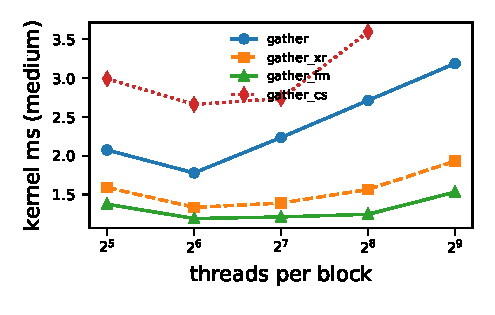
\includegraphics[width=\columnwidth]{figures/ir2_blocks.pdf}
\caption{Block-size sweep on the medium instance (median of 10). gather\_cs stops at 256 threads, where its shared memory reaches 33 KB per block.}
\label{fig:blocks}
\end{figure}



\subsection{Setup}

One Colab session on a Tesla T4 (40 SMs, 320 GB/s, CUDA through CuPy 14.0.1) ran
\file{notebooks/ir2\_colab.ipynb}, which carries a snapshot of the code, runs the unit tests (64 passed)
and then \file{bench/ir2.py}. The three synthetic sizes are those of IR1: small (2,000 genes by 20,000
cells, 3.2 M nonzeros), medium (4,000 by 50,000, 16.0 M) and large (8,000 by 120,000, 76.8 M), all with
$D = K = 30$. Kernel times are CUDA-event medians of three interleaved trials of ten launches and
include the row normalisation. Every kernel output was compared with a float64 reference before it
was timed. All six methods passed on all sizes, with a maximum relative error of $1.3 \times 10^{-6}$.
The complement kernel has the largest error among the gather variants ($1.2 \times 10^{-6}$ against
$2.2 \times 10^{-7}$), as expected from computing a sum as a difference.

\subsection{Idea 1: the layout on the GPU}

Table~\ref{tab:layout} shows the GPU layout 12 to 15 times faster than the host code, and on every size
its four arrays are bit-for-bit equal to the host ones. It is short of the 10 to 30 ms I estimated for
medium (43 ms), because the estimate counted memory traffic only, while the build runs about a dozen
library calls (sorts, binary searches, the cuSPARSE transpose) that each make a full pass over 16 million
64-bit indices.

End to end (Table~\ref{tab:e2e-medium}), the gather pipeline falls from 670 ms to 130 ms on medium, a
5.2$\times$ gain against the 7 to 9$\times$ I predicted, and now beats the single-thread C++ reference
(296 ms in IR1) by 2.3$\times$. It still loses to scatter (62 ms), and the breakdown says why. The layout
is now only 38 ms. The largest stage is the copy of the raw inputs (57 ms, against 32 ms for the IR1
arrays), because \code{GpuRaw} converts $X$ to CSC and sends $S$ as 64-bit indices, and the second
largest is a host step I had not looked at: computing the donor code of each cell with \code{np.unique}
over string labels (31 ms). The same pattern holds on large (Table~\ref{tab:e2e-large}), 2.58 s down to
0.57 s, behind scatter's 0.40 s. So the idea did what it was meant to do, and the bottleneck has moved to
data preparation that the real pipeline does not need: the R export already stores donors as integer
factor codes, and 32-bit selection indices would halve the size of $S$.

\subsection{Idea 3: fused mask stream and transposed reduction}

\paragraph{The first attempt failed, and why.} In the first run the transposed reduction was written
as a loop over the offset $o$ with an inner loop of length $o$. Both kernels that used it were
4 to 5$\times$ \emph{slower} than the baseline (7.9 and 8.8 ms against 1.7 ms on medium). The ptxas
report showed a 128-byte stack frame for both, exactly 32 floats: nvcc had not unrolled the nested
loop, so \code{acc[]} was indexed at run time and moved to local memory. Nsight confirmed it. DRAM
throughput rose from 29\% to 66\%, warp cycles per issued instruction from 10.9 to 49, while the
instruction count fell from 161 M to 95 M. The reduction was doing what it should, and the spill was
eating the gain. Writing each halving step as a template on a compile-time offset (\code{halve<O>})
removed the stack frame (0 bytes, 65 registers, the same as the baseline). All numbers below are from the
second run, with that fix.

\paragraph{Results.} On small and medium the fused kernel is 1.84$\times$ and 1.42$\times$ faster than
the IR1 gather (Table~\ref{tab:kernels}), inside the 1.4 to 2$\times$ range estimated in
Section~\ref{sec:ideas}. The ablation separates the two parts. The transposed reduction alone
(\code{gather\_xr}) gives 1.68$\times$ and 1.32$\times$, so most of the gain is the reduction, and the
fused mask stream adds 9 to 15\% on top.

\paragraph{A new dimension: where the instructions and bytes went.} Table~\ref{tab:ncu2} lists Nsight
counters for one launch of each kernel on medium. The transposed reduction halves the instruction count
(161 M to 80 M), close to the 1.8$\times$ fewer adds I predicted. Fusing the mask leaves the instruction
count where it is but cuts the bytes the L1 handles from 656 MB to 269 MB, 2.4$\times$ less, which
matches the claim that the dependent lookup was most of the L1 traffic. DRAM bytes read stay at about
235 MB in all three kernels, which shows that the mask lookups had been served from cache all along.
With both changes the kernel is no longer instruction-bound: DRAM throughput is at 70\%, against 30\%
for the baseline, and warp cycles per instruction fall from 10.9 to 8.6. The kernel has moved most of
the way from the SM roof to the memory roof, so further gains on this layout must come from reading
fewer bytes per nonzero.

\paragraph{Large.} On large the gain disappears: 4.92 against 4.94 ms, and \code{gather\_xr} is slower
(6.7 ms). I cannot fully explain this from the data I have. Large timings were noisy on this shared GPU,
with trial medians of the baseline ranging from 4.9 to 7.1 ms. In the fastest trials the fused kernel
still led (4.27 against 4.86 ms). Two effects are plausible. Large segments are 2.4 times longer (320
nonzeros against 133), so the reduction, which the fusion mostly fixes, is a smaller share of the
work. And at 8 bytes per nonzero the fused kernel reads 614 MB, so its DRAM floor is about 1.9 ms,
which leaves less room. Nsight was only run on medium, so profiling large is the first item of the next
step.

\paragraph{Block size.} Figure~\ref{fig:blocks} sweeps the block size on medium. Every gather variant is
fastest at 64 threads, two warps per block. The fused kernel is the least sensitive (1.19 to 1.53 ms
across the sweep), because with no dependent load each warp needs fewer others to hide its latency.
128 threads, used everywhere else, costs 2 to 26\% depending on the kernel.

\subsection{Idea 2: complement accumulation}

\paragraph{The work cut is real.} Table~\ref{tab:work} counts the work from the actual layouts. The
flip marks 643 of the 900 pseudo-bulks on medium, the set bits per cell fall from 18.8 to 8.7, and the
adds per nonzero from 32 to 9.7, 3.3$\times$ fewer, exactly as estimated from $\mathbb{E}[\min(r,1-r)]$.
Because a warp waits for its slowest lane, the lane steps fall by only 2.2$\times$: the mean of the
warp-wide maximum is 13.5 set bits, against a mean of 8.7. Nsight agrees on the direction. The kernel
executes 110 M instructions against 161 M.

\paragraph{The time is worse.} Despite that, \code{gather\_cs} is 0.87$\times$, 0.51$\times$ and
0.46$\times$ the speed of the baseline. My estimate (0.8 to 1.3$\times$) was too optimistic on medium
and large. Table~\ref{tab:ncu2} shows three causes, in order of size.
(1) \emph{Occupancy.} The 16.9 KB of shared accumulators per 128-thread block allow three blocks per SM,
and achieved occupancy drops from 84\% to 34\%. With a quarter of the warps resident, the latency of the
shared-memory read-modify-write is no longer hidden. (2) \emph{Bank conflicts.} Lanes write to rows
chosen by their data, and Nsight counts 21.6 M bank conflicts in one launch. (3) \emph{Divergence.}
Active threads per instruction drop slightly, from 22.4 to 21.0 out of 32, because lanes leave the \code{\_\_ffs}
loop at different times. So the PRAM cost model is right about the work but misses what SIMT charges
for it: a lockstep warp pays for its slowest lane, and moving accumulators out of registers trades
arithmetic for latency.

\paragraph{New ideas from this result.} The analysis points to two fixes. (a) Keep the accumulators
in registers and use the complement only to make the masks sparser, splitting each warp's 32
accumulators into the flipped and unflipped halves so that a loop step only visits the half with set
bits. The work cut then survives without shared memory. (b) If shared memory stays, give each lane a
private, conflict-free column (the read layout already is) and launch two-warp blocks, which the block
sweep already favours. I expect (a) to matter more, because occupancy, not conflicts, is the largest
loss.

\subsection{Against a library}

cuSPARSE SpGEMM through \code{cupyx} computes the same product correctly but takes 81 ms on small and
324 ms on medium, about 210 and 270 times slower than the fused kernel, and it runs out of memory on large
(it asked for 36 GB). A general sparse-sparse product does not know that each row of $S$ touches one
donor or that the output is dense, so it forms and merges every partial product. The donor layout uses
both facts, which is where the advantage over the general routine comes from. This matches the
pseudo-bulk literature, where the step is done as a generic sparse product in R or
Python~\cite{crowell2020,squair2021}.


\section{Future work}

The Final Report rubric asks for inputs bigger than device memory and for tensor or RT cores.
\begin{enumerate}
\item \textbf{Bigger than memory.} The donor layout splits naturally by gene. Blocks of genes can be
streamed through the device with the copy of one block overlapping the kernel of the previous one, and
each block's output is independent.
\item \textbf{Tensor cores.} Per donor, $PB_d = M_d X_d^{\top}$, with $M_d$ the dense $K \times n_d$
0/1 matrix and $X_d$ the donor's $n_d \times G$ slice. The 0/1 operand is exact in FP16, so dense
tiles of $X_d$ could go through tensor cores where the data is dense enough to pay for the zeros.
\item \textbf{Real data.} Run everything on the real matrix exported from Narval, where uneven cells
per donor and nonzeros per cell will make segment lengths uneven.
\item \textbf{More than 32 pseudo-bulks per donor}, with several mask words.
\end{enumerate}

\section{Conclusion}

Profiling the IR1 code showed that its pipeline was host-bound and its kernel was bound by on-chip work,
not DRAM. Moving the layout to the GPU fixed the first (5.2 times end to end on medium), and the fused
kernel moved the second most of the way to the memory roof (1.4 times, DRAM throughput from 30\% to
70\%). The complement idea showed that a cut in PRAM work does not survive SIMT costs when it pushes
accumulators out of registers, which sets the next step: keep the work cut in registers, profile the
large input, and remove the host-side preparation that now dominates the pipeline.

\bibliographystyle{ACM-Reference-Format}
\bibliography{refs}

\end{document}
